\documentclass{standalone}
\usepackage{calc}
\usepackage{tikz}
\usepackage{hsbcommon}
\begin{document}
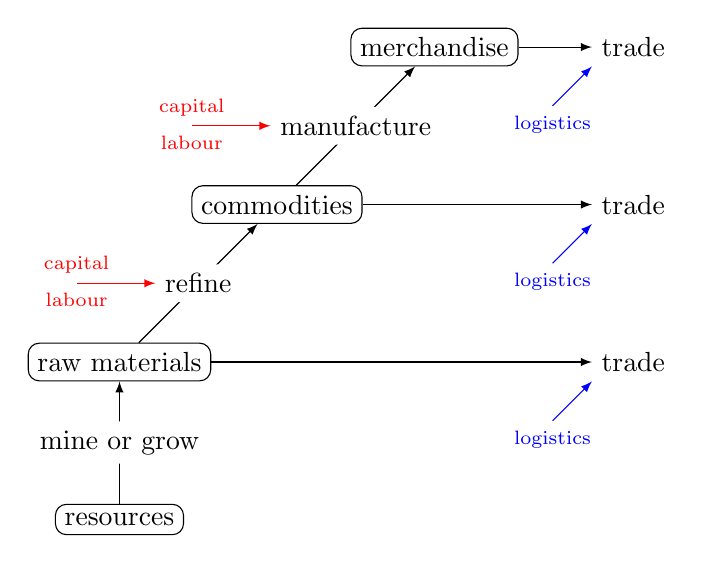
\begin{tikzpicture}
    \tikzset{every node/.style={rounded corners}}
    
    \node[draw, rounded corners] (re) at (0,-2) {resources};
    \node[draw, rounded corners] (rm) at (0,0) {raw materials};
    \node[draw, rounded corners] (com) at (2,2) {commodities};
    \node[draw, rounded corners] (merch) at (4,4) {merchandise};
    \draw[->,>=latex]  (re) -- node[fill=white] (mine) {mine or grow} (rm);
    \draw[->,>=latex]  (rm) -- node[fill=white] (refine) {refine} (com);
    \draw[->,>=latex] (com) -- node[fill=white] (manufacture) {manufacture} (merch);
    \foreach \i in {rm,com,merch} {\draw[->,>=latex] (\i) -- (6,|- \i) node[right] (t\i) {trade}; } 

    \ifstep{2}{
\begin{scope}[color=red]

        \draw[<-,>=latex]  (refine.west) -- ++ (-1,0) node[above] {\scriptsize capital} node[below] {\scriptsize labour};
        \draw[<-,>=latex]  (manufacture.west) -- ++ (-1,0) node[above] {\scriptsize capital} node[below] {\scriptsize labour};
    \end{scope}
}

    \ifstep{3}{
\begin{scope}[color=blue]

        \foreach \i in {rm,com,merch} {
            \draw[<-,>=latex] (t\i.south west) -- ++ (-0.5,-0.5) node[below] (t\i) {\scriptsize logistics}; 
            } 
    \end{scope}
}

\end{tikzpicture}
\end{document}
